%\begin{savequote}[75mm]
%The individual is ephemeral, races and nations come and pass away, but man remains.
%\qauthor{Nikola Tesla}
%\end{savequote}

\chapter{Tópicos Específicos}
	\label{ch:topicos_selectos}

Dentro de este capítulo se abordan técnicas y mecanismos que modelan el comportamiento de la arquitectura propuesta para aceleradores basados en múltiples núcleos de procesamiento. Si el lector no se encuentra familiarizado con los conceptos básicos de redes en-chip, se recomienda cubrir el material presentado en el capitulo \ref{chap:fundamentos}, en particular las secciones \ref{sec:redes_de_interconexion} y \ref{sec:conceptos_basicos_de_nocs}, antes de internarse en este capítulo.

\begin{figure}
	\begin{center}
		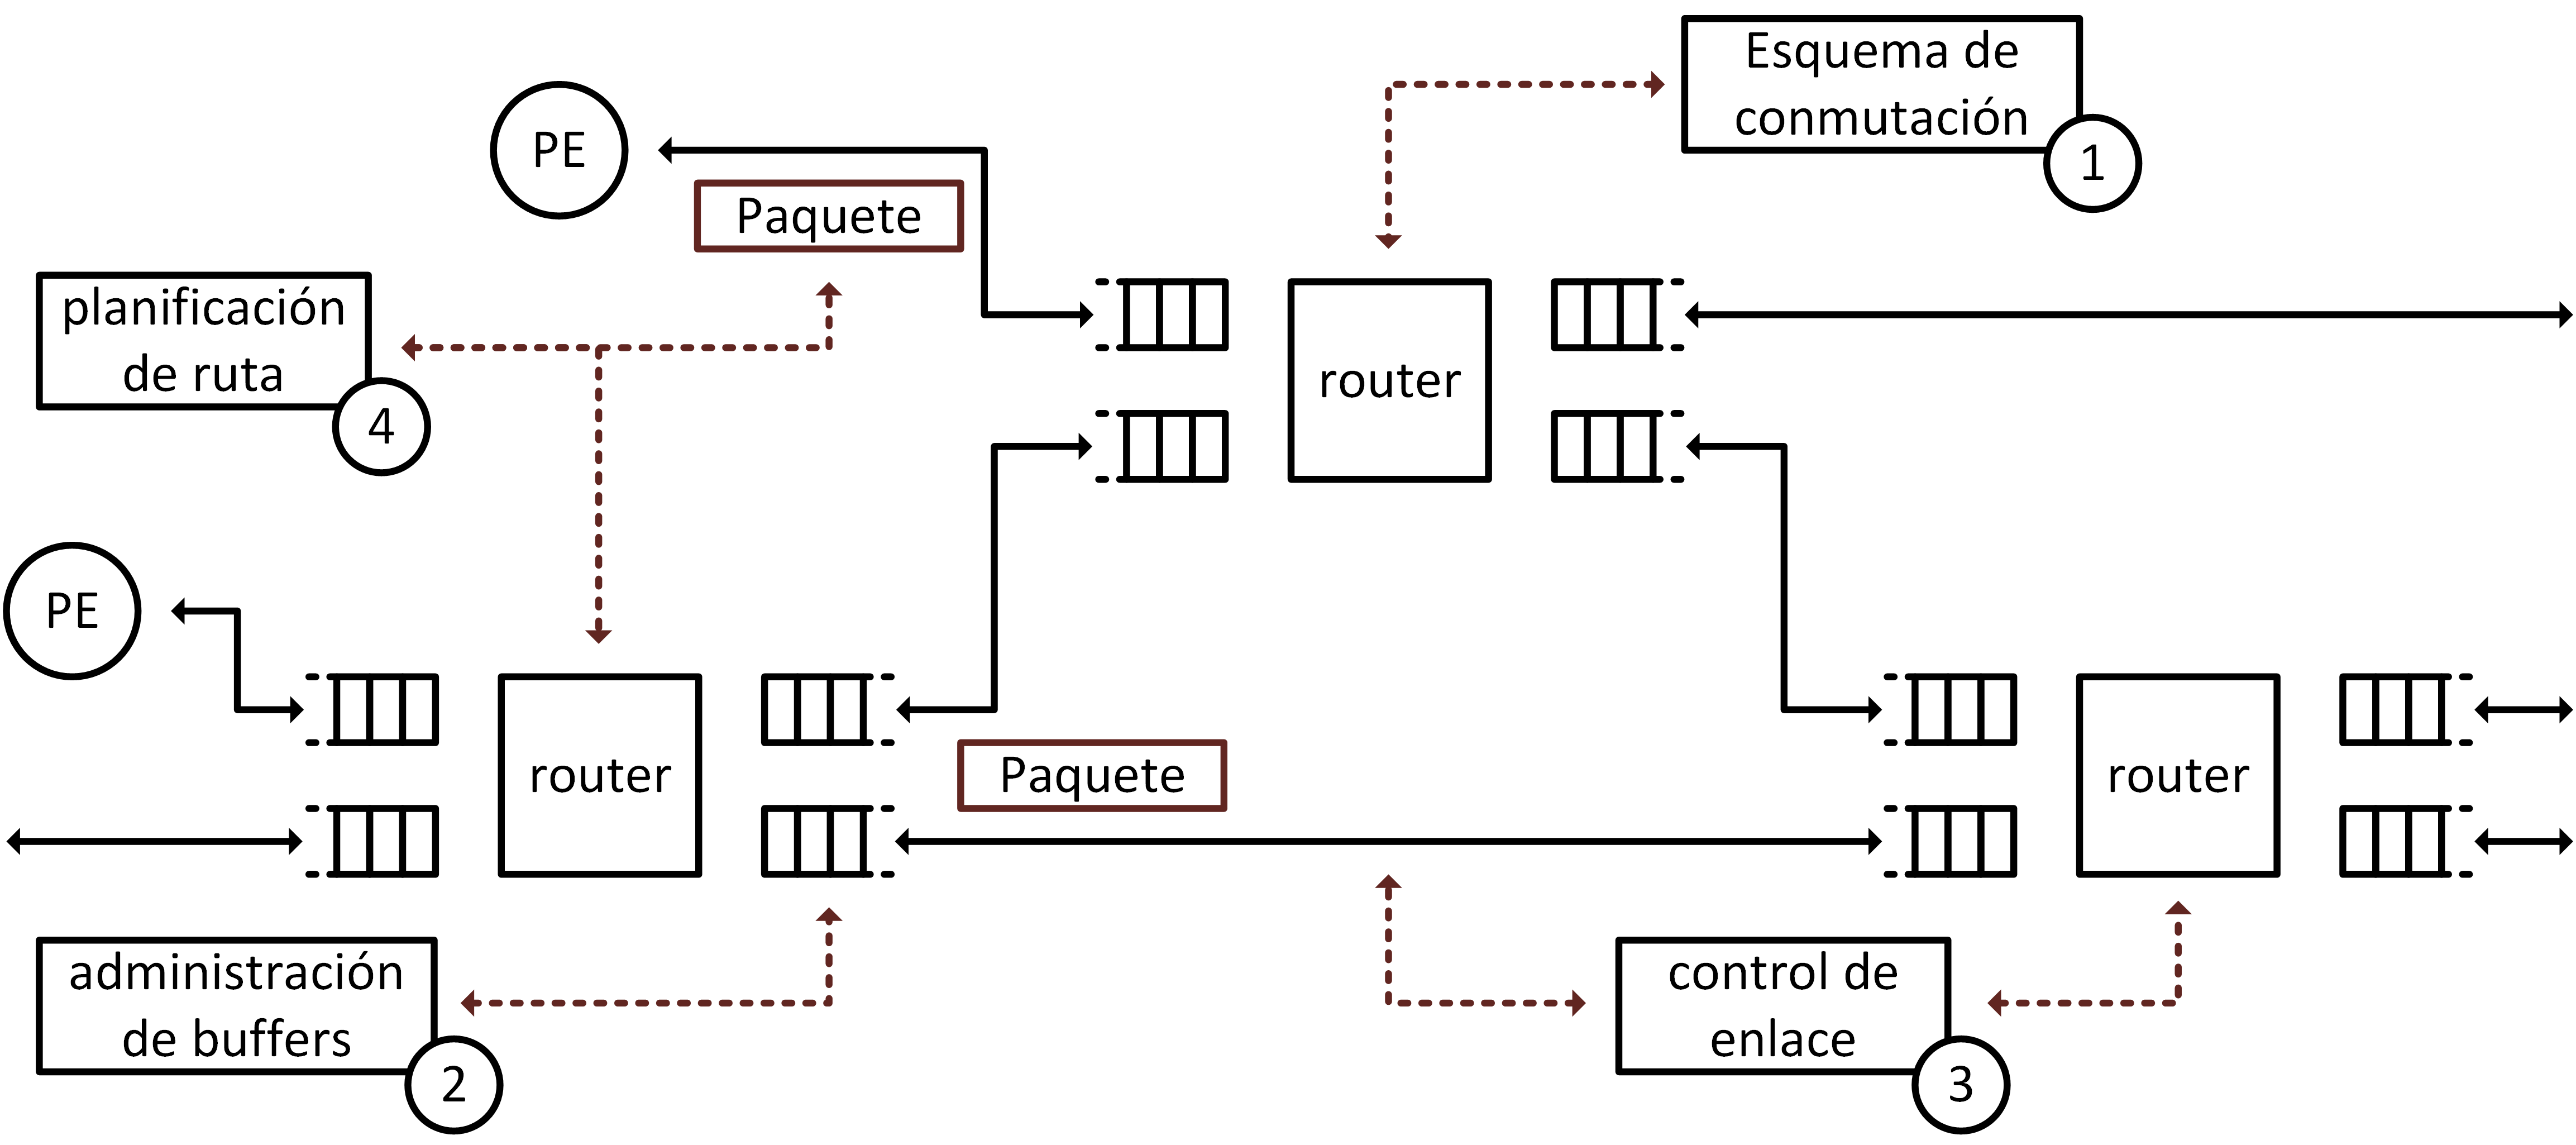
\includegraphics[scale = 0.5]{figures/ch2_topicos_general.png}
	\end{center}
	\caption
		{	
			Diagrama abstracto de una red en-chip. \textit{PE} representa un Elemento de Procesamiento. La figura resalta los módulos de la red impactados por los parámetros descritos dentro de este capitulo.  
		}
	\label{fig:ch2_topicos_general}
\end{figure}

La figura \ref{fig:ch2_topicos_general} muestra una representación abstracta de una red en-chip. Dentro de esta figura se indica los módulos impactados por los mecanismos tratados en esta sección. El contenido de este capítulo se desarrolla en el siguiente orden: en primer lugar se abordan las características para redes organizadas con una topología tipo malla. De manera subsecuente se describen las técnicas de control de flujo para la arquitectura propuesta en este trabajo. El control de flujo se lleva a cabo a nivel de administración de buffers, puntos 1 y 2 de la figura \ref{fig:ch2_topicos_general}, y a nivel de enlace, punto 3 de la misma figura. La sección posterior ofrece una visión general de la familia de algoritmos basados en el \textit{modelo basado en giros} o \textit{turn model}. Los algoritmos de planificación de ruta impactan al módulo con el cual comparten nombre, localizados en la figura bajo el punto 4. Cabe mencionar que este capítulo no muestra detalles de la micro arquitectura de la red, el capitulo \ref{chap:nodo_de_red} abarca dicho nivel de detalle.



\section{Topología: Malla} 
	\label{sec:topologia_malla}
	


Una red con topología tipo malla alberga $N = k^2$ nodos en una cuadricula regular de dos dimensiones, donde cada dimension contiene $k$ nodos con enlaces solo a sus vecinos inmediatos. Una malla presenta una organización regular, con canales de comunicación entre nodos de longitud reducida que facilita su colocación en silicio. La figura \ref{fig:ch2_mesh_caracteristicas} presenta una malla con 16 nodos.

Las mallas son redes asimétricas respecto a sus vértices, ya que los nodos en la periferia presentan un menor grado de colectividad respecto los nodos centrales (figura \ref{fig:ch2_mesh_caracteristicas} c)). La asimetría de la topología puede producir desbalances en la distribución de tráfico en la red, ya que los canales centrales tendrán mayor demanda con respecto a los canales de la periferia ya que los primeros forman parte de un mayor numero de rutas entre nodos. Al ser una topología asimétrica el grado de nodo no es homogéneo para todos sus miembros, sin embargo es una practica común definir $\delta = 4$ para todos los nodos de la red y dejar sin conexión los canales sin vecino inmediato\footnote{Los puertos sin conexión son optimizados por las herramientas de síntesis para código de descripción de hardware (HDL en ingles)} como se muestra en la figura \ref{fig:ch2_mesh_caracteristicas} c).

\subsection{Desempeño de una malla}

Factores como topología, control de flujo y algoritmo para la planificación de ruta determinan la capacidad de una red para el desplazamiento de información entre sus miembros, el máximo flujo de datos es denominado rendimiento de la red ($\Theta$). En el resto de esta sección se presenta el desempeño ideal de una red tipo malla así como los factores que lo determinan. Los datos presentados en esta sección utilizan la configuración de red de la figura \ref{fig:ch2_mesh_caracteristicas}. 
 
\begin{figure}
	\begin{center}
		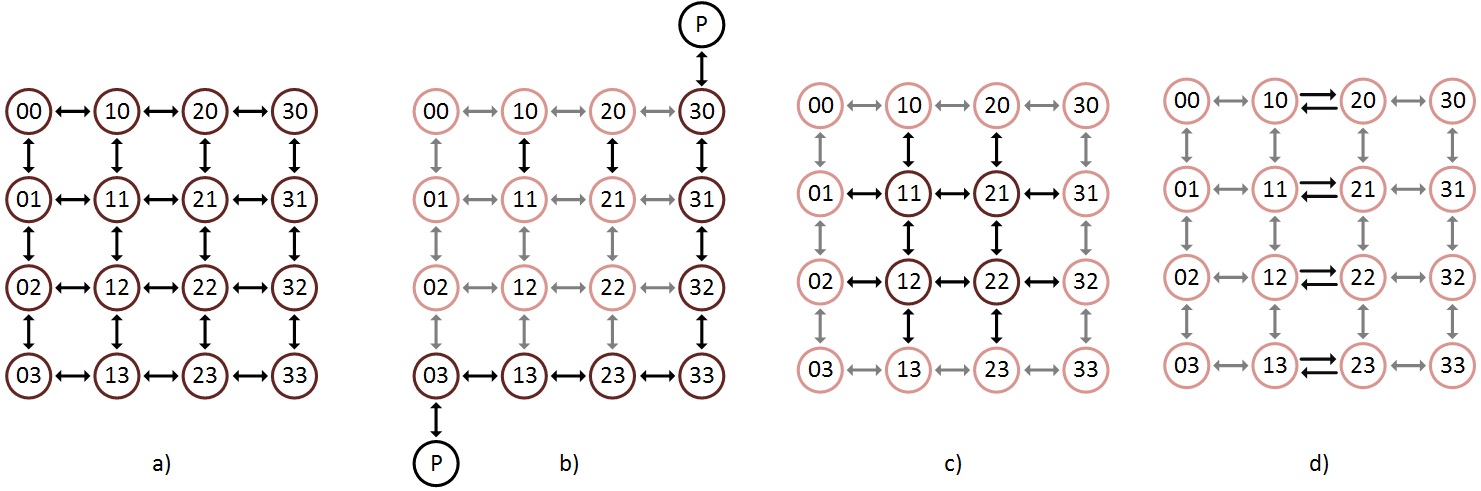
\includegraphics[scale = 0.6]{figures/ch2_mesh_caracteristicas.png}
	\end{center}
	\caption
		{	
			Topología tipo malla. a) red con topología tipo malla, a cada nodo se le asigna una dirección compuesta de una tupla $(x,y)$. b) Número de saltos requeridos para comunicar los elementos de procesamiento más distantes de la red. c) Los nodos al centro de la red tienen el mayor \textit{grado} de conectividad. d) Ancho de banda en la bisección.
		}
	\label{fig:ch2_mesh_caracteristicas}
\end{figure}

El rendimiento de una red es la relación entre el ancho de banda disponible y la demanda de transporte de información. El máximo rendimiento de la red se presenta cuando uno de sus canales alcanza el estado de saturación, es decir, la carga de trafico en el canal ($\gamma_{c}$) es igual al ancho de banda del mismo. El rendimiento ideal de una red se representa como la relación en la ecuación \ref{ecu:ch2_rendimiento}.

\begin{equation}
	\label{ecu:ch2_rendimiento}
		\Theta_{ideal} = \dfrac{b}{\gamma_{max}} 
\end{equation}

En la ecuación anterior $\gamma_{max} = max\left(\gamma_{C}\right)$. Para la red en la figura \ref{fig:ch2_mesh_caracteristicas}, bajo un esquema  de trafico uniforme, en todo momento la mitad de los paquetes en transito (${N/2}$) deben pasar a través de la bisección. El numero de canales que forman parte de la bisección de una malla esta definida por la ecuación \ref{ecu:ch2_biseccion}\footnote{Para redes tipo malla el numero de dimensiones $n$ es igual a $2$.} y se representa gráficamente en la figura \ref{fig:ch2_mesh_caracteristicas} d). Si el trafico en la bisección se encuentra distribuido de manera igualitaria entre los nodos que la forman, la máxima carga entre canales de la red esta definida como la carga de trafico en los canales de la bisección (\ref{ecu:ch2_carga_biseccion}).

\begin{equation}
	\label{ecu:ch2_biseccion}
		B_{c} = k^{n-1}
\end{equation}

\begin{equation}
	\label{ecu:ch2_carga_biseccion}
		\gamma_{B} = \dfrac{N}{2B_{C}}
\end{equation}

Para el caso particular de la malla bajo trafico uniforme, la carga máxima de trabajo esta definida por la carga en cualquiera de los canales que forman la bisecciòn de la red\footnote{Para redes tipo malla $2k^{n-1} = N/k$, siempre y cuando solo se encuentre un elemento de procesamiento por nodo.}

\begin{equation}
\label{ecu:ch2_carga_malla}
	\begin{split}
		\gamma_{M,U} &= \dfrac{N}{2k^{n-1}} \\
		             &= \dfrac{N}{2} \cdot \dfrac{1}{2k^{n-1}} \\
		             &= \dfrac{N}{2} \cdot \dfrac{k}{2N} \\
		             &= \dfrac{k}{4}
	\end{split}
\end{equation}

La ecuación de rendimiento requiere el ancho de banda para el canal que define $\gamma_{max}$. El ancho de banda esta determinado por la frecuencia de operación del router así como el ancho de canal del mismo, para una red tipo malla el ancho de canal esta definido por la ecuación \ref{ecu:ch2_ancho_de_canal}.

\begin{equation}
	\label{ecu:ch2_ancho_de_canal}
		W_{M} = \dfrac{W_{n}}{\delta_{n}}
\end{equation}

Sustituyendo las ecuaciones \ref{ecu:ch2_carga_malla} y \ref{ecu:ch2_ancho_de_canal} en la ecuación \ref{ecu:ch2_rendimiento} obtenemos:

\begin{equation}
	\label{ecu:ch2_rendimiento_malla}
		\begin{split}
			\Theta_{ideal, M} &= \dfrac{b}{\gamma_{max}} \\
			               &= \dfrac{fW_{M}}{k/4} \\ 
			               &= \dfrac{B_{n}/\delta_{n}}{k/4} \\
			               &= \dfrac{4B_{n}}{n\cdot k} 
		\end{split}
\end{equation}

Donde $B_{n} = f \cdot W_{M}$ representa el ancho de banda de un nodo de una malla.

\subsection{Latencia de una malla}

No solo el rendimiento de una malla determina el desempeño de esta como medio de transporte de información, otro factor a tomar en cuenta es la latencia entre el envió-recepción de un paquete. Una malla es una topología con un numero de dimensiones moderado ($n = 2$), por lo que el tiempo de transporte entre origen/destino esta dominado por el numero de saltos entre nodos.

El mínimo numero de saltos en una malla se calcula mediante el promedio de la distancia mínima entre todos los pares posible de nodos en la red. En promedio un paquete deberá visitar una tercera parte del total de nodos en cada dimension, por lo tanto el numero mínimo de saltos puede obtenerse mediante la ecuación:

\[ H_{min,M} =
  \begin{cases}
    \dfrac{nk}{3}       				& \quad \text{si } k \text{ es par}\\
    n\bigg(\dfrac{k}{3} + \dfrac{1}{3k}\bigg)	& \quad \text{si } k \text{ es inpar}\\
  \end{cases}
\]

La latencia no solo esta compuesta por el numero de saltos entre nodos, un segundo componente a tomar en cuenta es la latencia derivada de la serialización de un paquete en situaciones donde el ancho de canal ($W_{n}$) no es suficiente para el envió de datos en una sola transacción. La latencia de serialización ($T_{s,M}$) es igual a la relación entre la longitud en bits de un paquete y el ancho de banda disponible para su transporte.

\begin{equation}
	\label{ecu:ch2_latencia_serial}
		\begin{split}
			T_{s, M} &= \dfrac{L}{b} \\
			         &= \dfrac{1}{f} max \bigg( \dfrac{\delta nL}{W_{n}} \bigg)
		\end{split}
\end{equation}




\section{Control de flujo}

El control de flujo de una red en-chip se encuentra distribuido a través de la lógica de sus encaminadores. El control se divide en dos secciones principales: administración de buffers y control a nivel de enlace. La técnica para la administración de buffers se encarga de definir la partición lógica del espacio físico en las estructuras de almacenamiento en los puertos de entrada de un router, además de determinar los recursos que se deben de asegurar antes de la retransmisión de un paquete. Por otra parte, la técnica de control a nivel de enlace define estrategias para sincronizar la transmisión / recepción de paquetes entre nodos de la red, priorizando la entrega de paquetes entre nodos, y la velocidad de transferencia de dichas transacciones.


\subsection{Control de flujo basado en paquetes: Virtual Cut-Throught}

La red en-chip de este trabajo utiliza la técnica \textit{virtual cut-through}\cite{chapter2:Kermani79:virtualcut-through} para la administración de buffers en sus routers. Otros trabajos se refieren a esta técnica simplemente como \textit{cut-through}, en gran medida para evitar ambigüedades respecto al uso del término canales virtuales. Este documento hará uso del término abreviado cut-through.

Cut-through divide de manera lógica los buffers en unidades de almacenamiento del tamaño de un paquete al igual que la técnica store \& forward, sin embargo, se caracteriza por su capacidad de tomar decisiones de planificación de ruta en el momento que se reciba la dirección del destino del mensaje. Aunado al proceso acelerado de resolución de ruta, es posible la propagación de los flits pertenecientes a un paquete de manera inmediata tras finalizar el proceso de cálculo de trayectoria y asignación de puerto de salida.

Otra de las características de la técnica en cuestión, es su dualidad de comportamiento dependiendo del estado de la ruta trazada para un paquete. Cuando la ruta se encuentra libre de bloqueos, el retardo de propagación de un paquete está definido por la siguiente expresión:

\begin{equation}
	t_{vct} = D(\Delta_{r} + \Delta_{s} + \Delta_{w}) + P[max(\Delta_{s}, \Delta_{w})]
	\label{eq:t_vct}
\end{equation}

Donde $\Delta_{r}$ representa el retardo de la lógica para la codificación y cálculo de ruta, $\Delta_{s}$ es el tiempo necesario para que un flit cruce el camino de datos del encaminador, $\Delta_{w}$ es el retardo de propagación de las pistas que forman un canal entre routers, $D$ es la distancia en saltos desde el nodo origen al nodo destino, y finalmente $P$, es el número de flits que conforman el paquete. En el segundo escenario, el paquete encuentra un bloqueo en su ruta, y debe de esperar a que el camino se despeje para continuar su tránsito. Para que la ecuación \ref{eq:t_vct} sea válida bajo un bloqueo en ruta, es necesario agregar un término con valor equivalente a la duración del bloqueo. Un router cut-through se comporta como un encaminador tipo wormhole durante bajas cargas de trabajo, debido a un número reducido de bloqueos a través de sus canales. Durante cargas altas de trabajo, el mismo router se comportara de manera similar a un encaminador store \& forward, capturando en su totalidad el paquete antes de realizar el reenvío del mismo.

Wormhole es la técnica más popular para el control de flujo en redes en-chip de propósito general, sin embargo, trabajos de investigación\cite{chapter2:Shin:1996:AIH:232665.232669, chapter2:Duato:2001:CRA:372836.372856} han documentado un rendimiento inferior de esta técnica frente a cut-through cuando se inyectan cargas de trabajo pesadas a la red. Gran parte de las disminución de rendimiento en redes wormhole se debe al relativamente bajo umbral de saturación derivado de la ocupación de múltiples routers cuando un paquete encuentra un bloqueo en su camino. Durante la saturación de una red cut-through, cuando un paquete se encuentra con un bloqueo, solo un router se ve afectado por la contingencia, mientras los demás canales y encaminadores operan de manera habitual. Vale la pena mencionar que la mayor eficiencia de redes cut-through bajo órdenes altos de trabajo requiere el pago de una penalización en área debido al incremento de espacio de buffer requerido en cada router. El tamaño estático de los paquetes de la red, descrita en este trabajo, limitan el impacto en área resultado de la implementación del control de flujo cut-through.

Una descripción gráfica del comportamiento de una transacción cut-through puede encontrarse en la figura \ref{fig:ch1_store_cut}.

\subsection{Control a nivel de enlace basado en créditos}
	\label{subsec:control_basado_creditos}

Se ha implementado una estrategia de control de flujo a nivel de enlace basado en créditos. El control basado en créditos requiere que cada nodo de la red mantenga un registro del espacio disponible en los buffers de recepción de paquetes de cada uno de sus vecinos inmediatos. El objetivo de este registro es el evitar la pérdida de paquetes debido a la falta de espacio para su recepción. Dado que se utiliza una administración de buffers tipo \textit{cut-through}, la unidad atómica de almacenamiento es el paquete, por lo que un crédito equivaldrá al espacio necesario para almacenar todos los flits de un paquete.

Durante un restablecimiento general de la red, cada uno de los routers inicia sus contadores de créditos con la cantidad de espacios disponibles en los buffers de cada uno de sus nodos vecinos. Con cada envió de paquete, el router decrementa su contador de créditos. Antes de iniciar una transmisión, el encaminador emisor es responsable de verificar que aún cuenta con créditos para realizar el envío de un paquete, en caso contrario, este debe de retenerlo hasta que el router receptor cuente con el espacio suficiente para la captura de los datos.

El retorno de créditos es el mecanismo para informar que un router receptor a liberado un espacio en su buffer, se hace uso de una señal dedicada entre nodos para esta tarea. Al momento de la recepción de un crédito, el encaminador emisor incrementa su contador de créditos. 

\begin{figure}
	\begin{center}
		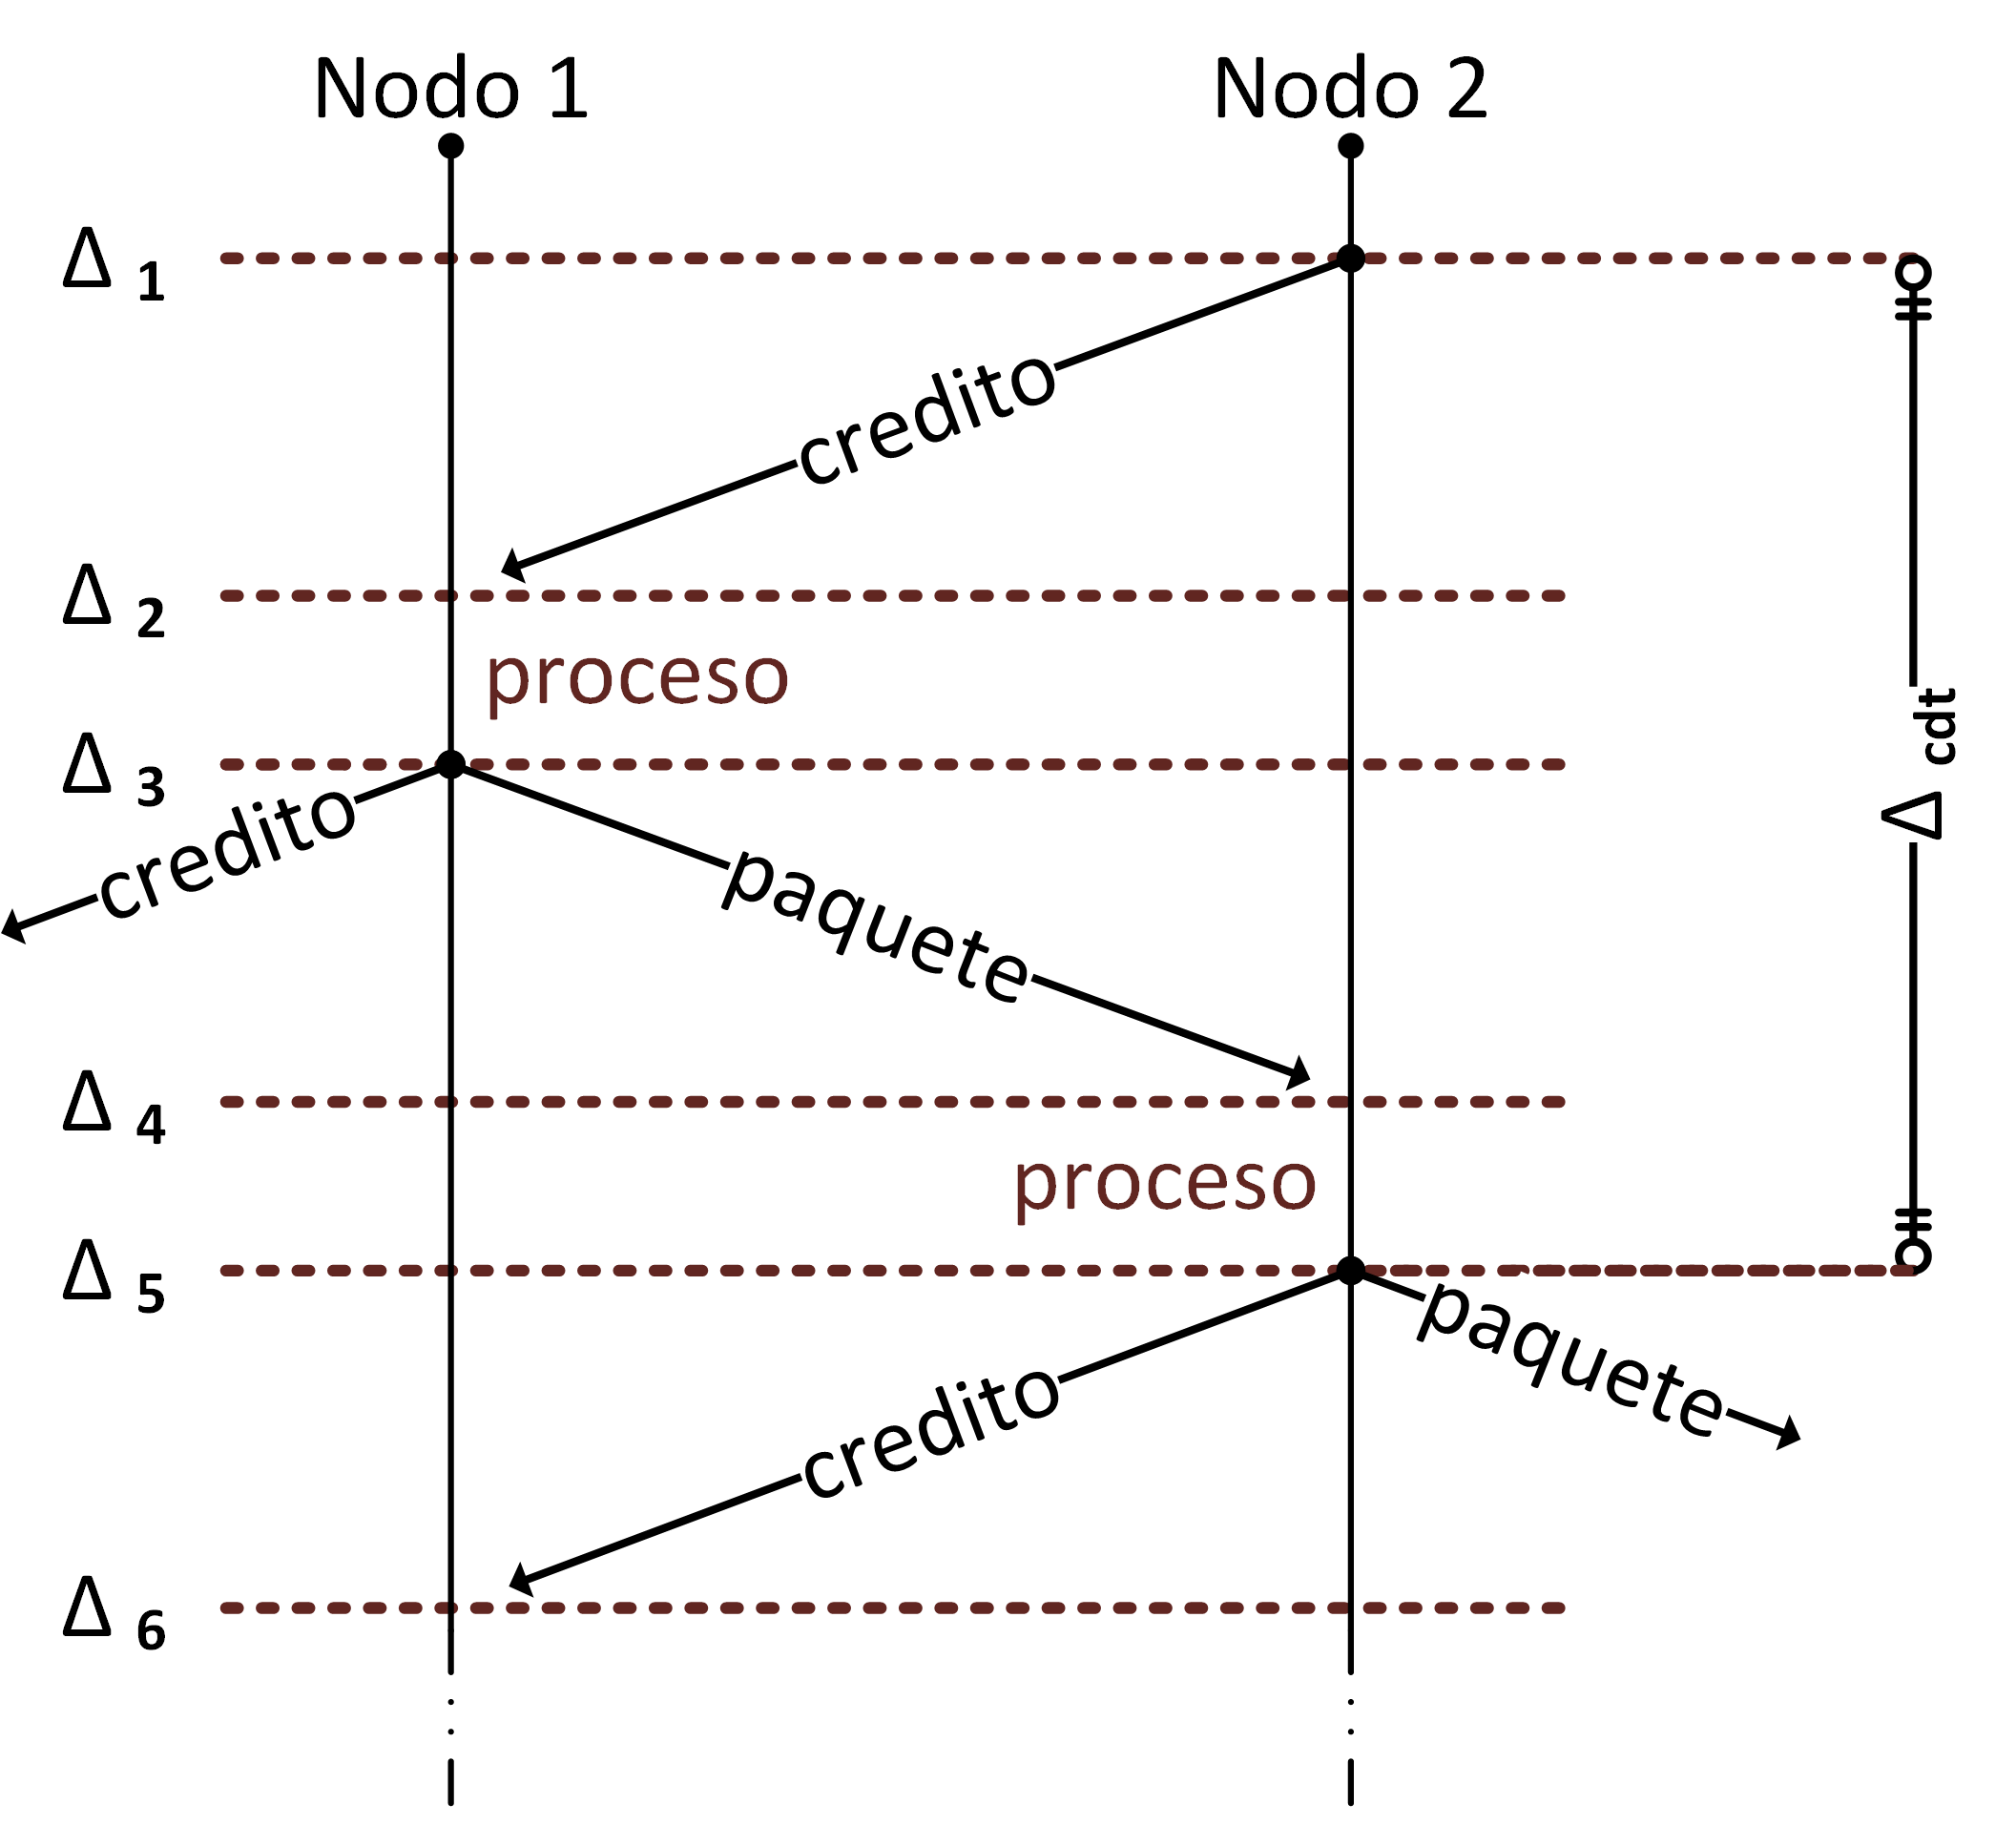
\includegraphics[scale=0.75]{figures/ch2_creditos_timeline.png}
	\end{center}
	\caption
		{	
			Línea de tiempo de proceso de transmisión de créditos. El nodo emisor (Nodo 1) resta un crédito con cada paquete que envía al nodo receptor. Cada crédito representa espacio de almacenamiento en los buffers del Nodo 2. El nodo receptor envía de vuelta un crédito con la salida de un paquetes de su medio de almacenamiento temporal. El escenario representado en esta figura supone nodos de red con espacio de almacenamiento suficiente para 1 solo paquete.
		}
	\label{fig:ch2_creditos_timeline}
\end{figure}

La figura \ref{fig:ch2_creditos_timeline} muestra el proceso de administración de créditos entre dos nodos de la red. El escenario inicia con la recepción en el nodo número 1 de un crédito durante $\Delta_2$. La recepción de un crédito implica el incremento en el contador interno del nodo, esta operación requiere un tiempo equivalente a $\Delta_3 - \Delta_2$. El nodo reconoce la recepción del crédito en $\Delta_3$, por lo que de manera inmediata reinicia la operación de envío de paquetes al nodo 2. La salida de un paquete del nodo 1 conlleva a la liberación de espacio en uno de sus buffers de recolección de paquetes, por lo que de manera simultánea con la salida del paquete en dirección del nodo 2 durante $\Delta_3$, el nodo 1 regresa un crédito al nodo origen del paquete que se acaba de transmitir. El nodo 2 recibe el último flit transmitido durante $\Delta_4$. El nodo 2 regresara un crédito al nodo 1 solo cuando libere el espacio ocupado por el paquete de reciente captura, este proceso puede llevar varios ciclos de reloj en caso de no contar con los recursos necesarios para reenviar el paquete a su destino. En este escenario, el nodo 2 no encuentra problemas para la retransmisión del paquete, por lo que después del tiempo necesario para la decodificación de la cabecera y la gestión de uso de recursos de salida, el paquete es liberado en dirección de su destino. El tiempo de gestión descrito anteriormente es equivalente a la diferencia $\Delta_5 - \Delta_4$. El tiempo $\Delta_{cdt}$, denominado \textit{tiempo mínimo de retorno de crédito}, es uno de los parámetros críticos para determinar el desempeño de un encaminador de red. $\Delta_{cdt}$ determina el tiempo necesario para completar un ciclo completo de retorno de un crédito para una misma posición en el buffer del nodo emisor. Para alcanzar un máximo rendimiento, un encaminador debe de proporcionar espacio suficiente en buffer para mantener transmisiones de paquetes de manera continua, sin interrupciones resultantes de la espera de devoluciones de créditos por parte del nodo receptor.

$\Delta_{cdt}$ limita la máxima tasa de transferencia entre nodos, por ejemplo, si un encaminador requiere de un crédito para el envió de un flit, y solo se cuenta con un crédito por puerto de entrada, la tasa de transferencia máxima estará modelada por la ecuación \ref{eq:bit_rate}.

\begin{equation}
	b_{cdt} = \frac{L_f}{\Delta_{cdt}}
	\label{eq:bit_rate}
\end{equation}

Donde $L_f$ representa la longitud en bits de cada paquete. La unidad de transferencia está dada en bits por segundo \textit{(bps)}. Generalizando la ecuacion \ref{eq:bit_rate} para modelar routers con mas de un espacio en buffer, se agrega el termino $F$ el cual representa el numero de espacios de recepción en el router objetivo. El incremento en el espacio de almacenamiento temporal permite el intercambio de un numero mayor de flits/paquetes antes de ser detenido el proceso debido a la falta de créditos. La tasa de transferencia de flits por $\delta_{cdt}$ se expresa en la ecuación \ref{eq:flits_cdt}.

\begin{equation}
	b_{flits} = F\frac{L_f}{\Delta_{cdt}}
	\label{eq:flits_cdt}
\end{equation}

De esta manera se calcula el número de buffers necesarios para garantizar la saturación de cada canal de la red, evitando el incremento de la latencia en el transporte de un paquete debido al tiempo de retorno de un crédito.

Para evitar una degradación del rendimiento es necesario proveer un mínimo de créditos para mantener una transferencia de paquetes constantes, se puede establecer relación en el numero de créditos respecto a $\delta_{cdt}$ mediante la ecuación \ref{eq:flits_cdt}:

\begin{equation}
	F \geq \frac{\Delta_{cdt}b_{cdt}}{L_{f}}
	\label{eq:flits_cdt}
\end{equation}


\section{Planificación de ruta: \textit{Modelo basado en giros}}

El modelo basado en giros\cite{chapter2:Glass:1998:TMA:285930.286003}, denominado  \textit{Turn model} en idioma inglés, ofrece un conjunto de reglas para la generación de algoritmos de encaminamiento para redes con topologías tipo malla o hipercubo. Los algoritmos obtenidos siguiendo los lineamiento de este modelo tienen la característica de ser parcialmente adaptativos, además de poder generar rutas mínimas o no mínimas.

El concepto de giro se refiere al cambio de dimensión durante el desplazamiento de un paquete a través de la red. La figura \ref{fig:ch2_turns} ejemplifica cada uno de los giros previstos por el modelo: Un giro simple se considera cualquier cambio de dimensión durante el traslado de un paquete, la figura \ref{fig:ch2_turns} apartado \textit{a)} refleja un giro de la dimensión \textit{x} a la dimensión \textit{y}, mientras que el apartado \textit{b)} representa un cambio desde la dimensión \textit{y} a la dimensión \textit{x}. El apartado \textit{c)} muestra un giro de 180°, se considera a este giro como un cambio de dirección mas no de dimensión. El giro de 0° no se encuentra ejemplificado en la figura \ref{fig:ch2_turns}, este giro representa un cambio de canal virtual dentro de la misma dirección y la misma dimensión. Si se requiere mayor información sobre este último tipo de giro se recomienda al lector la referencia de los autores \textit{Glass et. al.}

\begin{figure}
	\begin{center}
		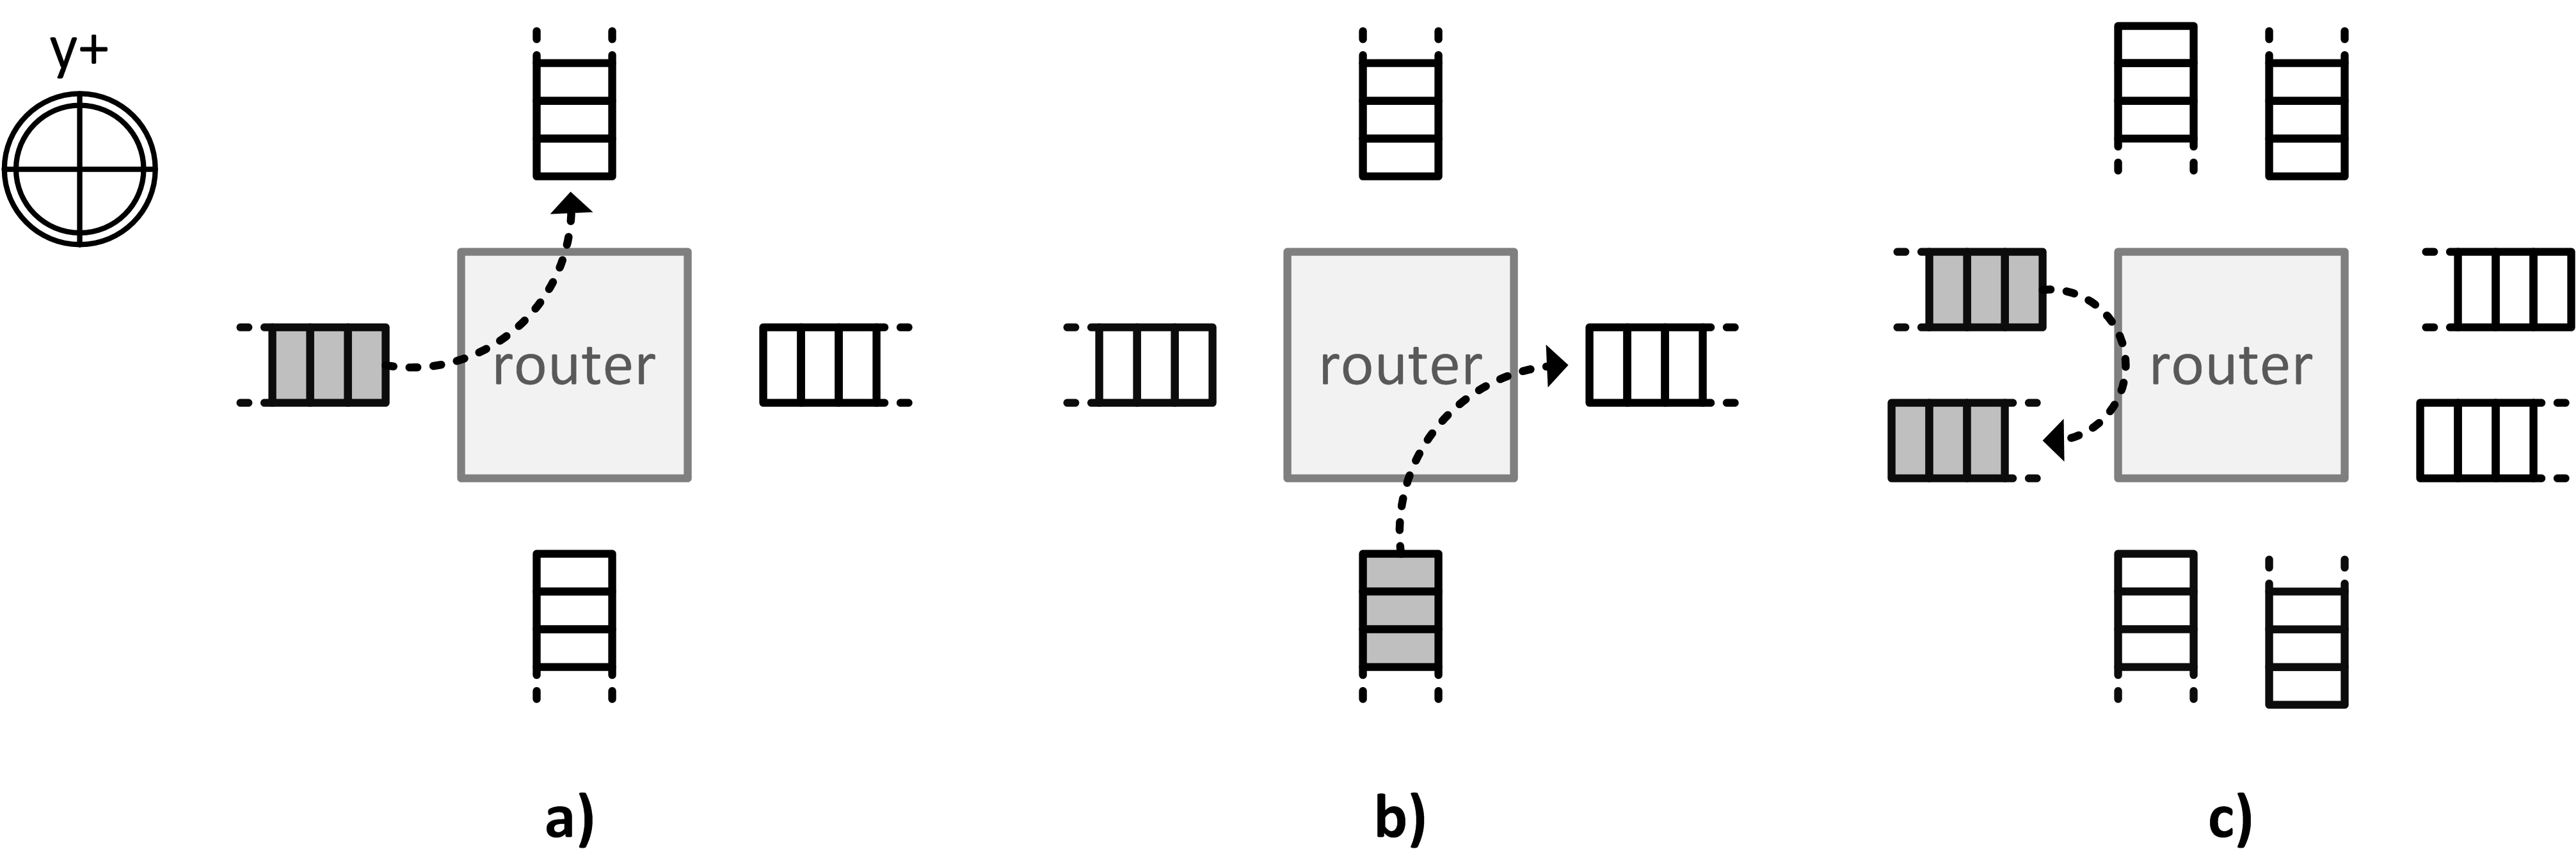
\includegraphics[scale=0.7]{figures/ch2_turns.png}
	\end{center}
	\caption
		{	
			Giros previstos durante una transferencia a través de la red.a) giro desde $x$ en dirección a $y$. b) giro desde $y$ en dirección a $x$. c) Giro de 180°, donde la dimensión de tránsito permanece sin alteración, sin embargo, la dirección de desplazamiento es alterada desde $x+$ a $x-$.
		}
	\label{fig:ch2_turns}
\end{figure}

El principal desafío de cualquier algoritmo de encaminamiento es el proveer de rutas libres bloqueos. Un bloqueo o \textit{deadlock}, se presenta cuando se forma una dependencia cíclica de peticiones de recursos entre paquetes como se muestra en la figura \ref{fig:ch2_giros_deadlock}. La estrategia empleada por el modelo basado en giros es el prohibir un subconjunto de giros posibles en la red de manera que se elimine toda posibilidad de creación de referencias cíclicas.

\begin{figure}
	\begin{center}
		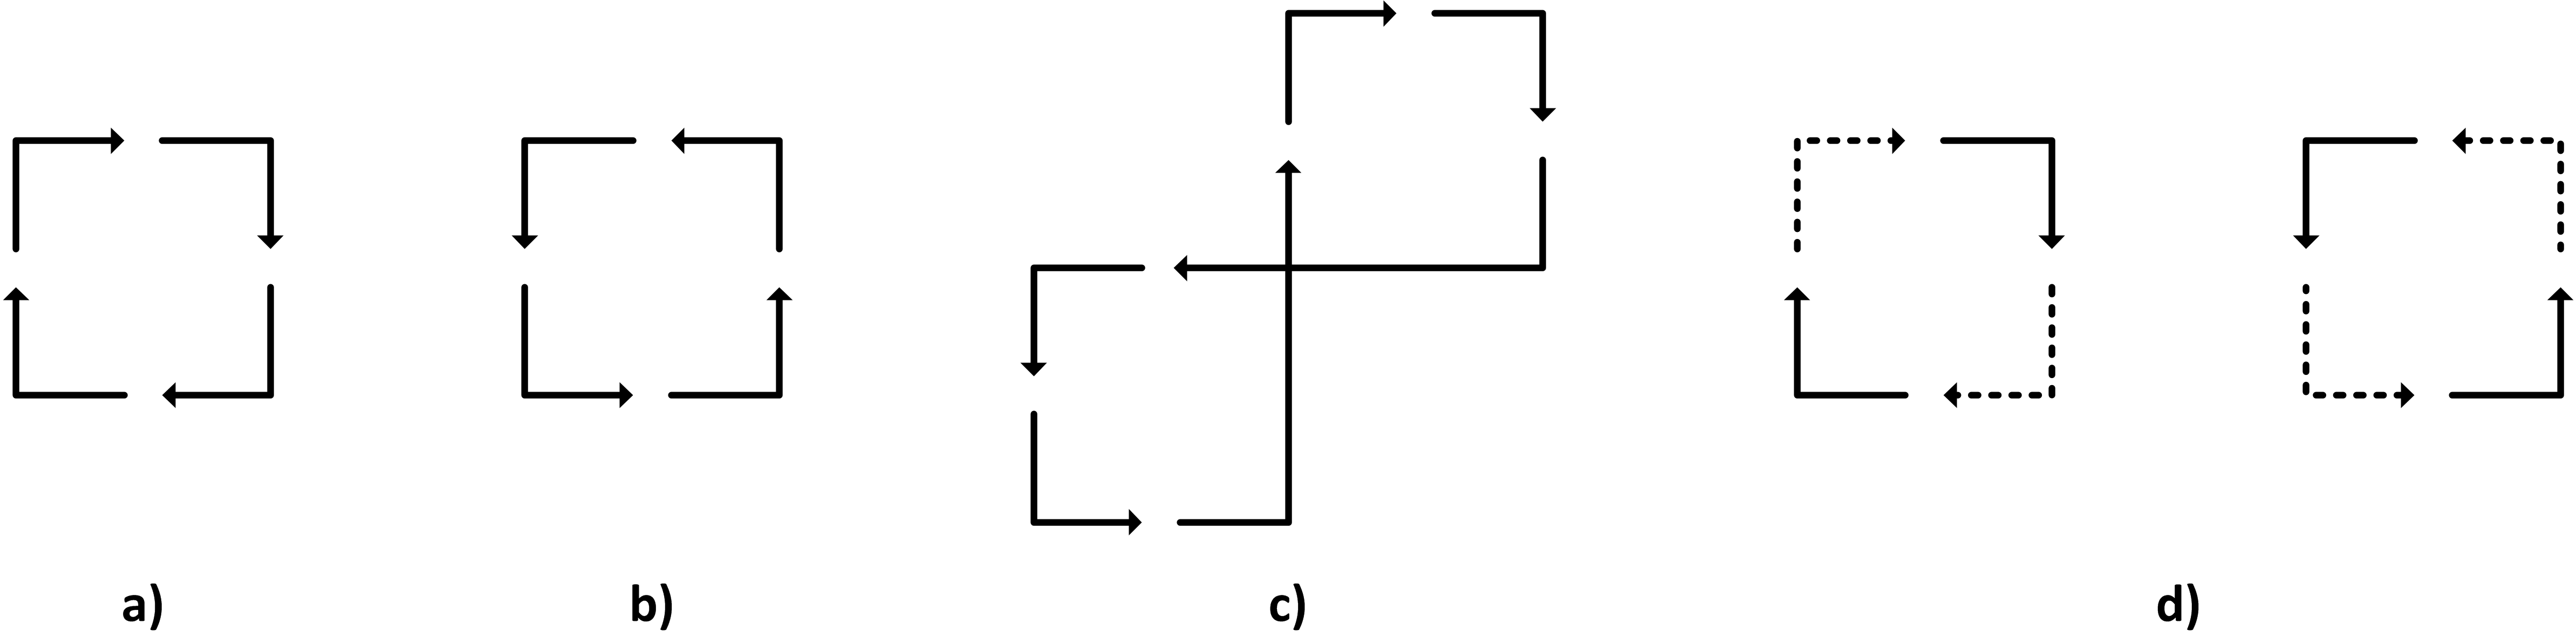
\includegraphics[scale=0.6]{figures/ch2_giros_deadlock.png}
	\end{center}
	\caption
		{	
			Posibles relaciones cíclicas en redes con topologías tipo malla. Los apartados a) y b) muestran la forma más simple de un \textit{deadlock}. El apartado c) muestra una dependencia cíclica compleja, la cual está formada por 6 giros y tránsito en direcciones opuestas. d) Giros prohibidos por el algoritmo XY para prevenir la formación de dependencias cíclicas.
		}
	\label{fig:ch2_giros_deadlock}
\end{figure}

La estrategia de prohibición de virajes no es única de los algoritmos desarrollados a partir del modelo basado en giros. El algoritmo XY\cite{chapter2:Shubhangi:2012} por ejemplo prohíbe los cuatro giros exhibidos en la figura \ref{fig:ch2_giros_deadlock} d) con la finalidad de evitar la creación de dependencias cíclicas. El modelo basado en giros tiene como fundamento un conjunto de pasos para la creación de nuevos algoritmos de ruteo. A continuación se lista un subconjunto de estos pasos, los cuales resultan de particular interés para topologías tipo malla:

\begin{enumerate}
	\item Clasificar cada canal de la red de acuerdo a la dimensión a la cual pertenece. Por ejemplo, en una malla 2d podemos clasificar los canales en las dimensiones \textit{x} o \textit{y}.
	\item Determinar los giros posibles en la red. Para mallas existen 8 giros distintos.
	\item Identificar todos las relaciones cíclicas que se pueden formar en la red, es importante verificar la existencia de ciclos formados a partir de combinaciones complejas de giros.
	\item Prohibir un giro de cada ciclo para evitar su formación.
\end{enumerate}

Si la red en-chip permite la inclusión de giros de 0° y 180°, estos se agregan después del punto 4 de la lista anterior y bajo la condición que la inclusión no genere nuevas dependencias que formen un ciclo.

\subsection{Grado de adaptabilidad}

Como se mencionó al inicio de esta sección, los algoritmos generados a partir del modelo basado en giros son parcialmente adaptativos. Cada algoritmo puede presentar diferentes grados de adaptabilidad, este último concepto se expresa mediante la ecuación:

\begin{equation}
	S_f = \frac{(\delta x + \delta y)!}{\delta x ! \delta y!}
	\label{eq:grado_adaptabilidad}
\end{equation}

Donde $S_{f}$ representa el numero de caminos cortos entre los nodos origen $(o_x, o_y)$ y destino $(d_x, d_y)$ ofrecidos por un algoritmo completamente adaptativo, $\delta x$ representa la diferencia $| d_x - o_x |$, y finalmente $\delta y = | d_y - o_y |$. Los algoritmos presentados en las siguientes sub secciones no pueden ofrecer el número máximo de caminos cortos en todas las direcciones de la red, por este motivo son considerados parcialmente adaptativos.


\subsection{Algoritmo West First minimal}
	\label{subsec:algoritmo_west_first_minimal}

El algoritmo \textit{west first minimal} prohíbe los giros $Y_{neg} \rightarrow X_{neg}$ y $Y_{pos} \rightarrow X_{neg}$, cada uno de estos giros rompe la posibilidad de crear una relación cíclica. Bajo west first, todos los paquetes deben de desplazarse en primer lugar en la dirección $X_{neg}$ en caso de ser necesario, ya que los giros para tomar esta dirección se encuentran prohibidos. Una vez terminado este desplazamiento inicial, el paquete puede ser encaminado de manera adaptativa hasta alcanzar su destino. El algoritmo \ref{code:west_first_minimal} ofrece un pseudocódigo para el encaminamiento tipo \textit{west first minimal}, esta descripción es capaz de manejar un paquete desde cualquier dirección inicial.

La ecuación \ref{eq:grado_wfm} modela el grado de adaptabilidad para el algoritmo west first. De acuerdo a esta ecuación, el área de la red que tiene capacidad de encaminar paquetes de manera adaptativa abarca todos los nodos que satisfacen la condición $d_x \ge o_x$. Esta condición resulta valiosa si se conoce el patrón de trafico que se espera en la NoC.

\begin{equation}
	\label{eq:grado_wfm}
S_{west-first}=\begin{cases}
    		\frac{(\delta x+\delta y)!}{\delta x! \delta y!}, & \text{si $d_x \ge o_x$}	\\
    		1,  & \text{en otros casos}\\
		\end{cases}
\end{equation}

La figura \ref{fig:ch2_wf_example} muestra 4 rutas calculadas mediante el algoritmo west first, 3 de estas rutas presentan bloqueos a través de la red mostrando la capacidad de adaptabilidad del encaminamiento de paquetes. El caso particular donde el paquete inicia en la esquina inferior derecha de la red  ejemplifica el peor de los casos para este algoritmo, ya que no se satisface la condición $d_x \ge o_x$. West first se implementa como un algoritmo de ruteo distribuido, por lo que cada nodo de la red toma sus propias decisiones de encaminamiento tomando en cuenta solo la información de trafico de sus vecinos inmediatos. Este último mecanismo permite tomar tomar rutas alternas inclusive cuando el camino inicial fuese el peor de los casos.

\begin{figure}
	\begin{center}
		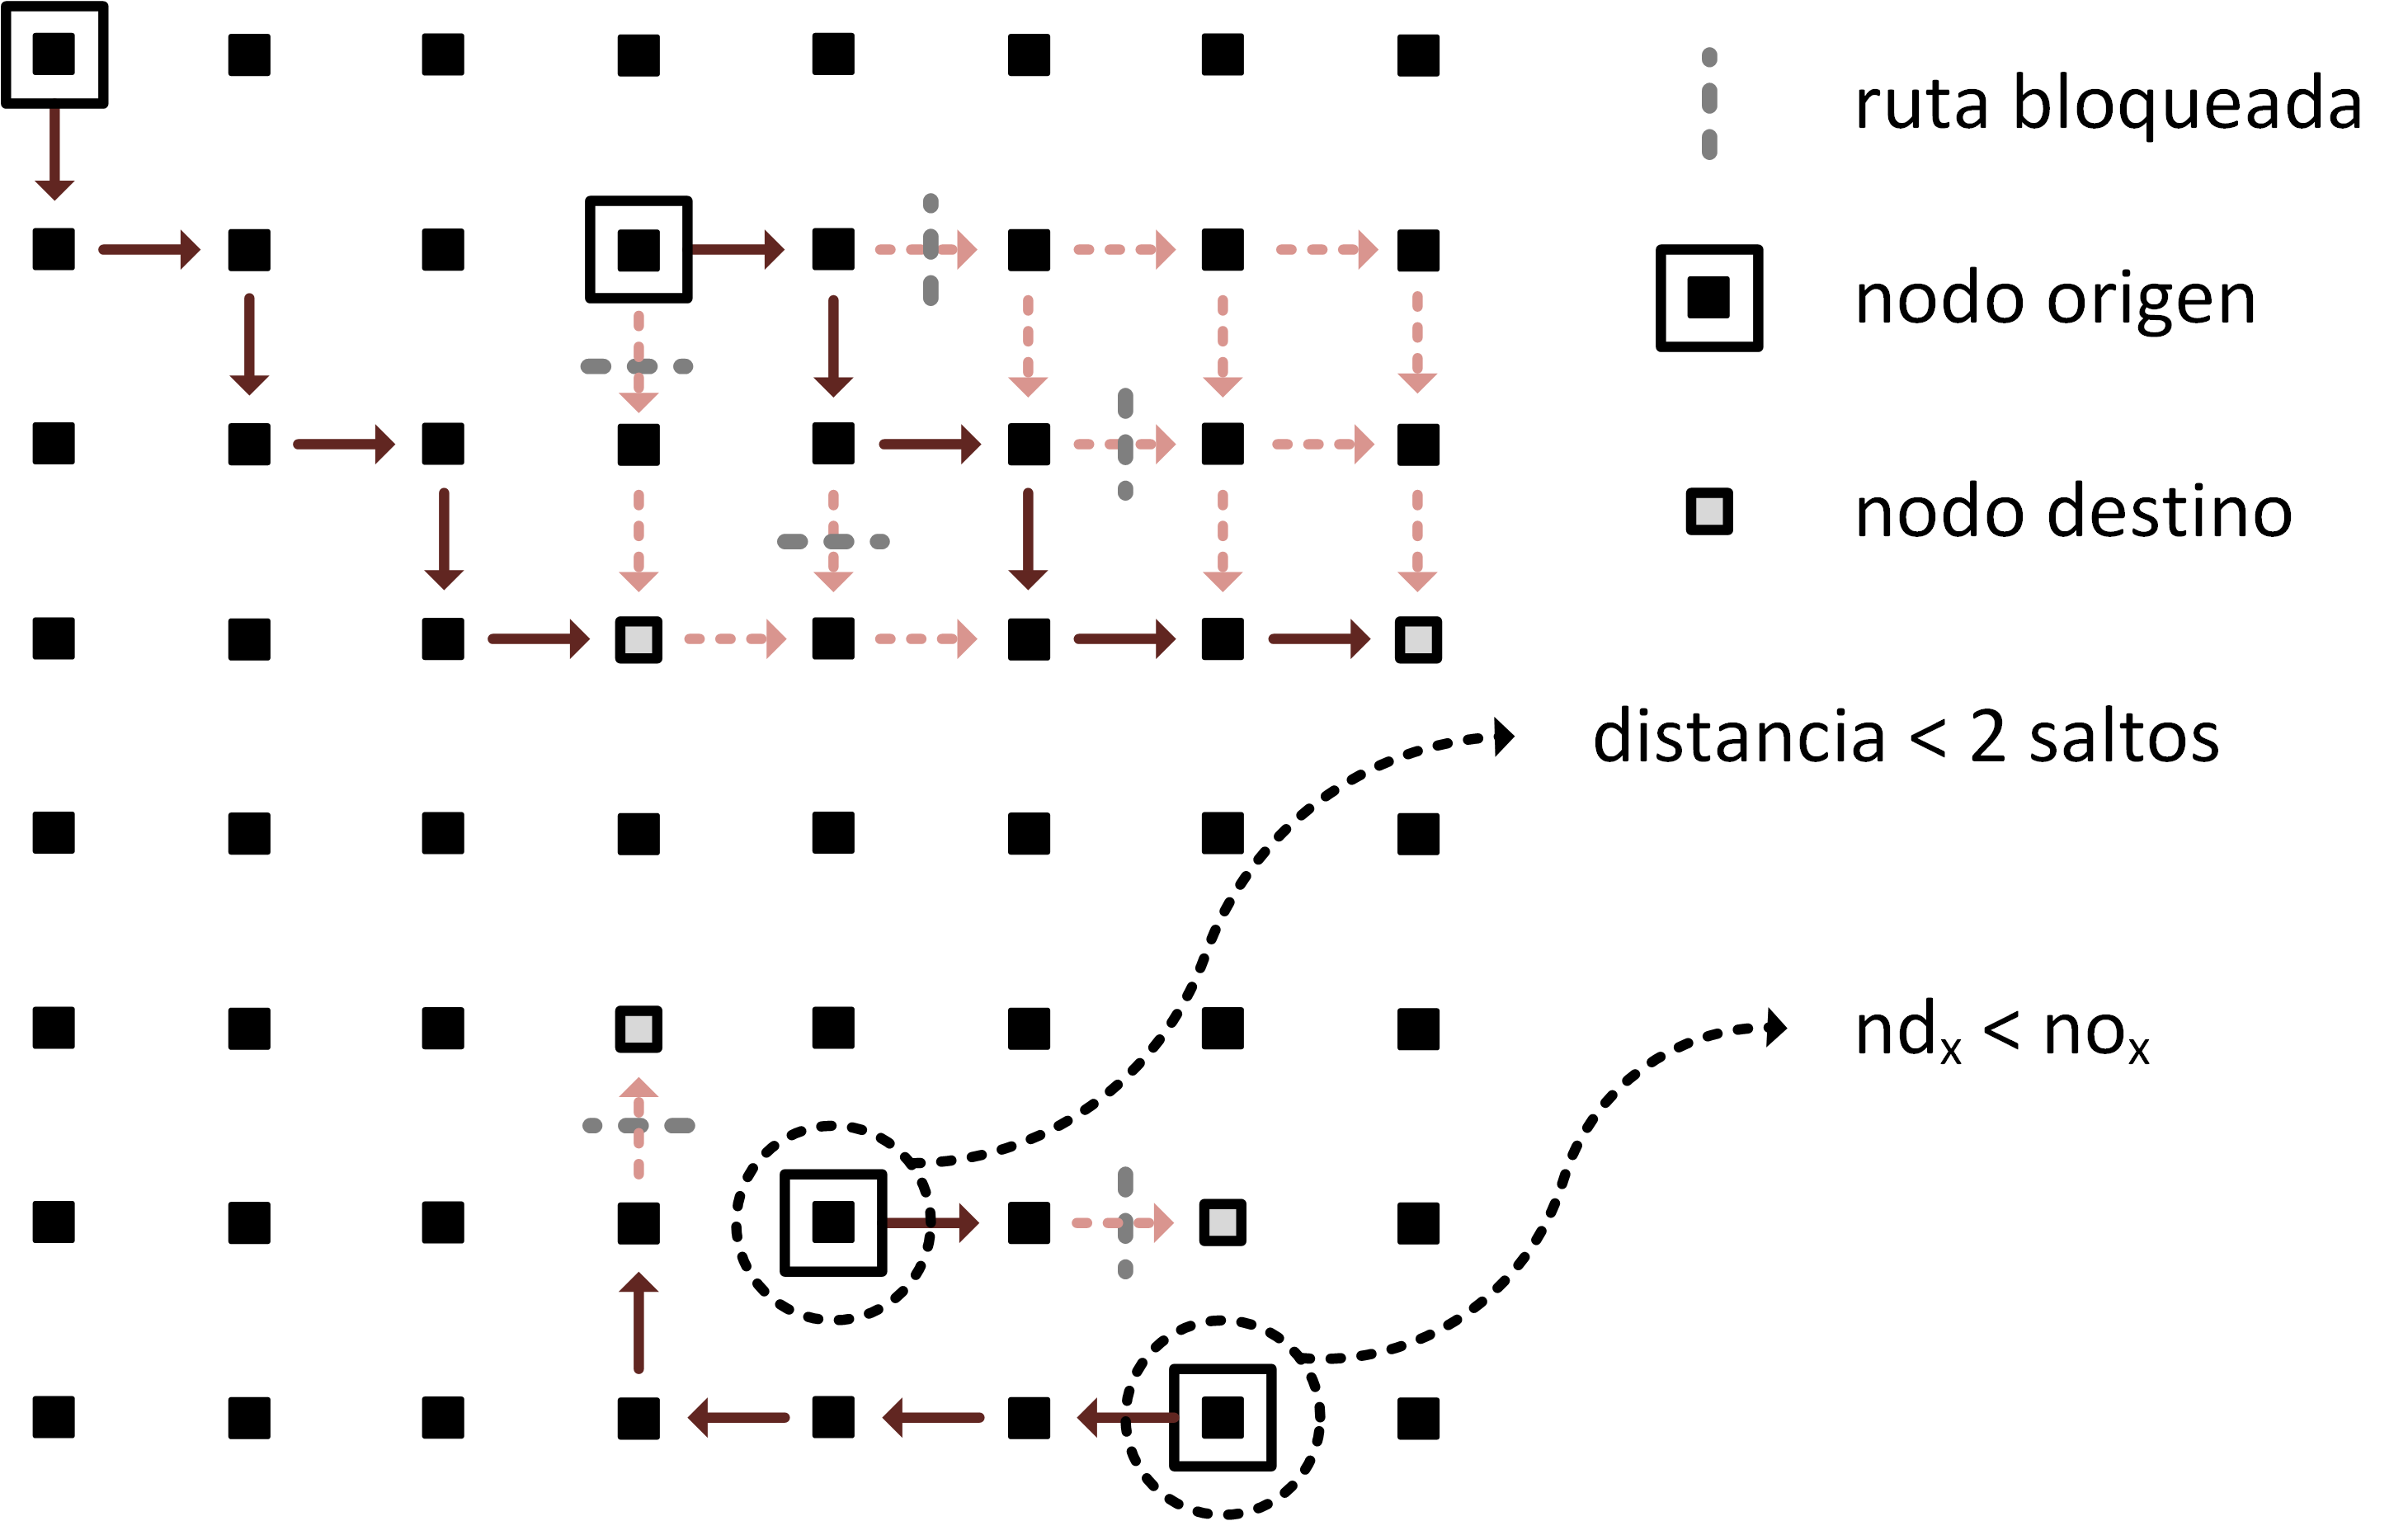
\includegraphics[scale=0.6]{figures/ch2_wf_example.png}
	\end{center}
	\caption
		{	
			Rutas planificadas por medio del algoritmo west-first minimal. Las rutas creadas por medio de este algoritmo permite sortear bloqueos gracias a su capacidad de adaptabilidad. La ruta con inicio en la esquina inferior derecha muestra los cambios de adaptabilidad de la ruta conforme es reevaluada en cada nodo de la red.
		}
	\label{fig:ch2_wf_example}
\end{figure}

\begin{algorithm}[]
	\KwData{\:\:dirección de nodo actual (\textit{localX}, \textit{localY})\\
			\Indp \Indp dirección de nodo destino (\textit{destX}, \textit{destY})}
	\KwResult{canales de salida válidos (\textit{canales})}
		\Begin
			{
			offsetX = destX - localX\;
			offsetY = destY - localY\;
				\If{offsetX < 0}
					{
						canales := X-\;
					}
				\If{offsetX > 0 \textbf{and} offsetY < 0}
					{
						canales := (X+, Y-)\;
					}
				\If{offsetX > 0 \textbf{and} offsetY > 0}
					{
						canales := (X+, Y+)\;
					}
				\If{offsetX > 0 \textbf{and} offsetY = 0}
					{
						canales := X+\;
					}
				\If{offsetX = 0 \textbf{and} offsetY < 0}
					{
						canales := Y-\;
					}
				\If{offsetX = 0 \textbf{and} offsetY > 0}
					{
						canales := Y+\;
					}
				\If{offsetX = 0 \textbf{and} offsetY = 0}
					{
						canales := elemento de procesamiento\;
					}
		}
	\caption
		{
			\textit{West-First minimal}
		}	
	\label{code:west_first_minimal}
\end{algorithm}